\documentclass[10pt]{beamer}

% ================== PACKAGES ==================
\usepackage{graphicx}
\usepackage{amsmath}
\usepackage{hyperref}
\usepackage{xcolor}

% ================== THEME ==================
\usetheme{Madrid}

% ----- GREY TITLE BAR & FOOTER ONLY -----
\definecolor{mygrey}{RGB}{120,120,120}

\setbeamercolor{frametitle}{fg=white,bg=mygrey}
\setbeamercolor{author in head/foot}{fg=white,bg=mygrey}
\setbeamercolor{title in head/foot}{fg=white,bg=mygrey}
\setbeamercolor{date in head/foot}{fg=white,bg=mygrey}

\setbeamercolor{normal text}{fg=black,bg=white}
\setbeamercolor{structure}{fg=black}

% ================== TITLE DETAILS ==================
\title[Landslide Detection]{Landslide Detection Using Deep Learning and Multispectral Satellite Images}
\author{Geethanjali Javvadi}
\institute{Department of ECE \\ GVPCEW Madhurawada}
\date{\today}

% ================== DOCUMENT ==================
\begin{document}
	
	% ---------- TITLE ----------
	\begin{frame}
		\titlepage
	\end{frame}
	
	% ---------- TOC ----------
	\begin{frame}{Table of Contents}
		\tableofcontents
	\end{frame}
	
	% =================================================
	% INTRODUCTION
	% =================================================
	\section{Introduction}
	
% ---------- PROBLEM STATEMENT ----------
% ---------- PROBLEM STATEMENT ----------
\begin{frame}{Problem Statement}
	
	% -------- IMAGES (TOP) --------
	\begin{center}
		\includegraphics[width=0.32\linewidth]{Landslide_image1.jpg}
		\hfill
		\includegraphics[width=0.32\linewidth]{Landslide_image2.png}
		\hfill
		\includegraphics[width=0.32\linewidth]{Landslide_image3.jpg}
	\end{center}
	
	\vspace{0.3cm}
	
	% -------- TEXT (BOTTOM) --------
	\begin{itemize}
		\item Landslides are among the most destructive natural disasters.
		\item They cause severe loss of:
		\begin{itemize}
			\item Human life
			\item Infrastructure
			\item Natural resources
		\end{itemize}
	
	\end{itemize}
	
\end{frame}


	\begin{frame}{Need for Automation}
		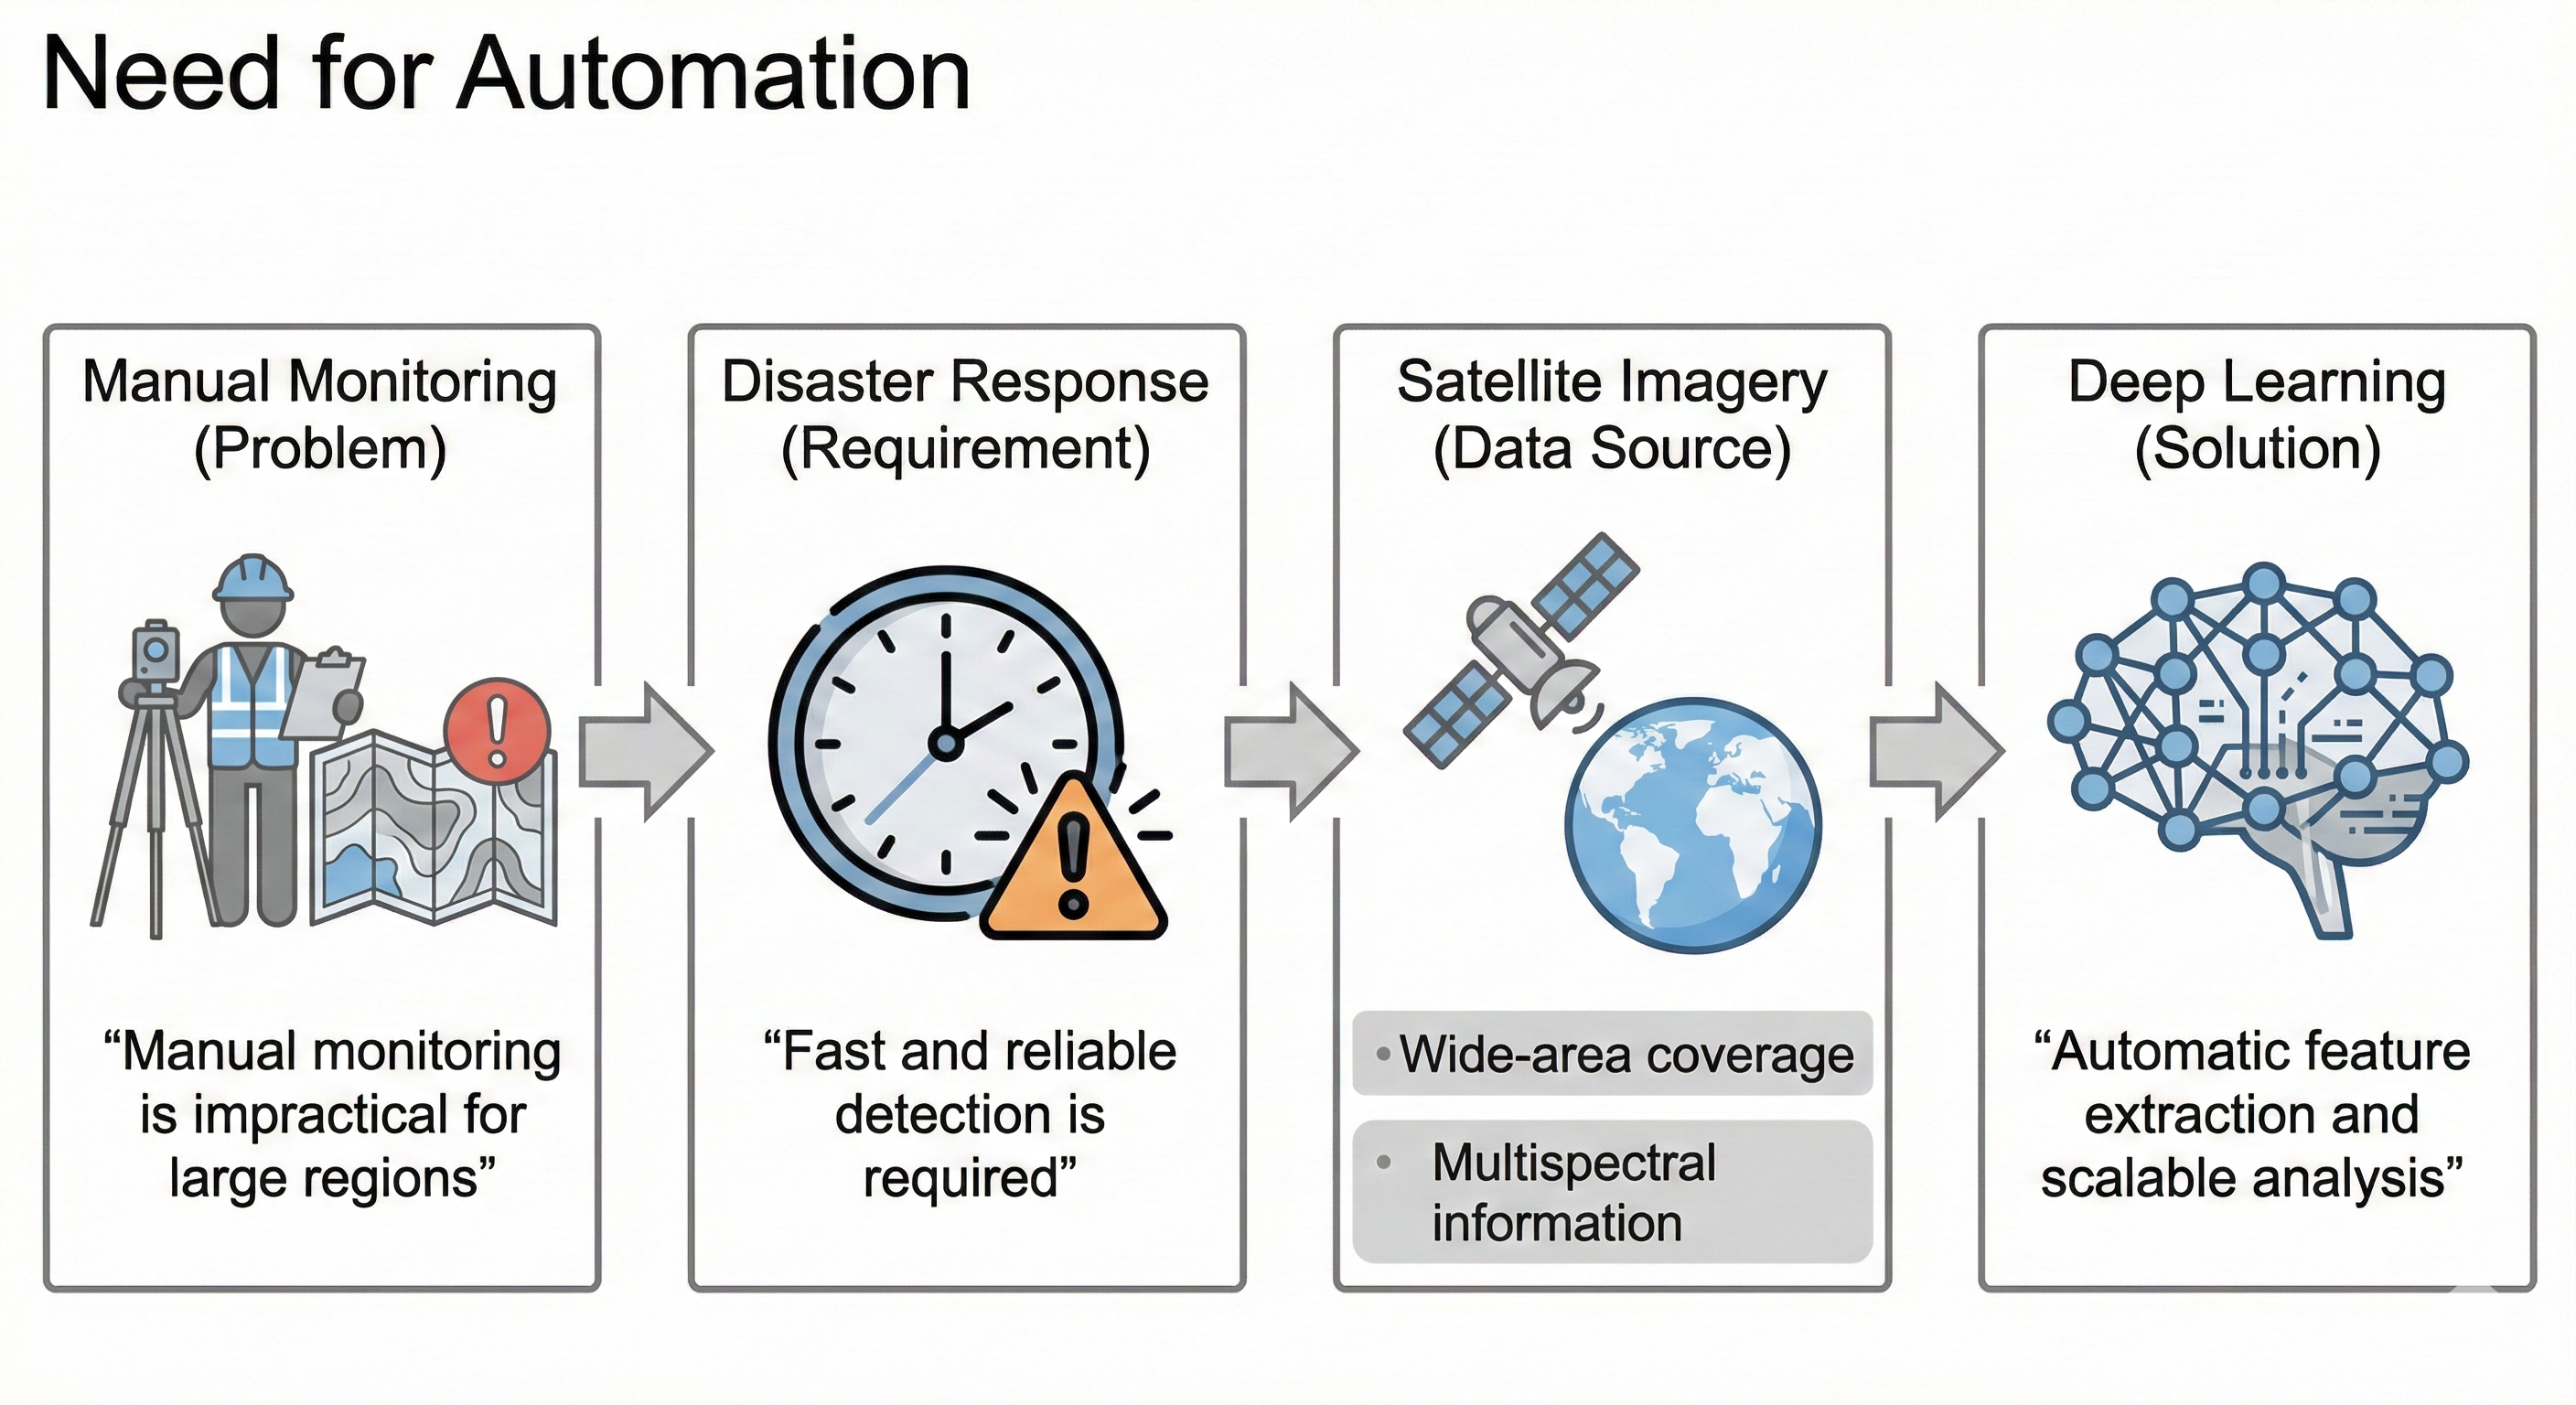
\includegraphics[width=0.9\linewidth]{need_for_automation.png}
		
		\begin{itemize}
			
			\item Manual monitoring is impractical for large geographical regions.
			\item Disaster response requires fast and reliable detection.
		\end{itemize}
	\end{frame}
	

	% ---------- PREVIOUS WORK ----------
	\section{Previous Work}
	\begin{frame}{Previous Work}
		
		% -------- IMAGE (TOP) --------
		\begin{center}
			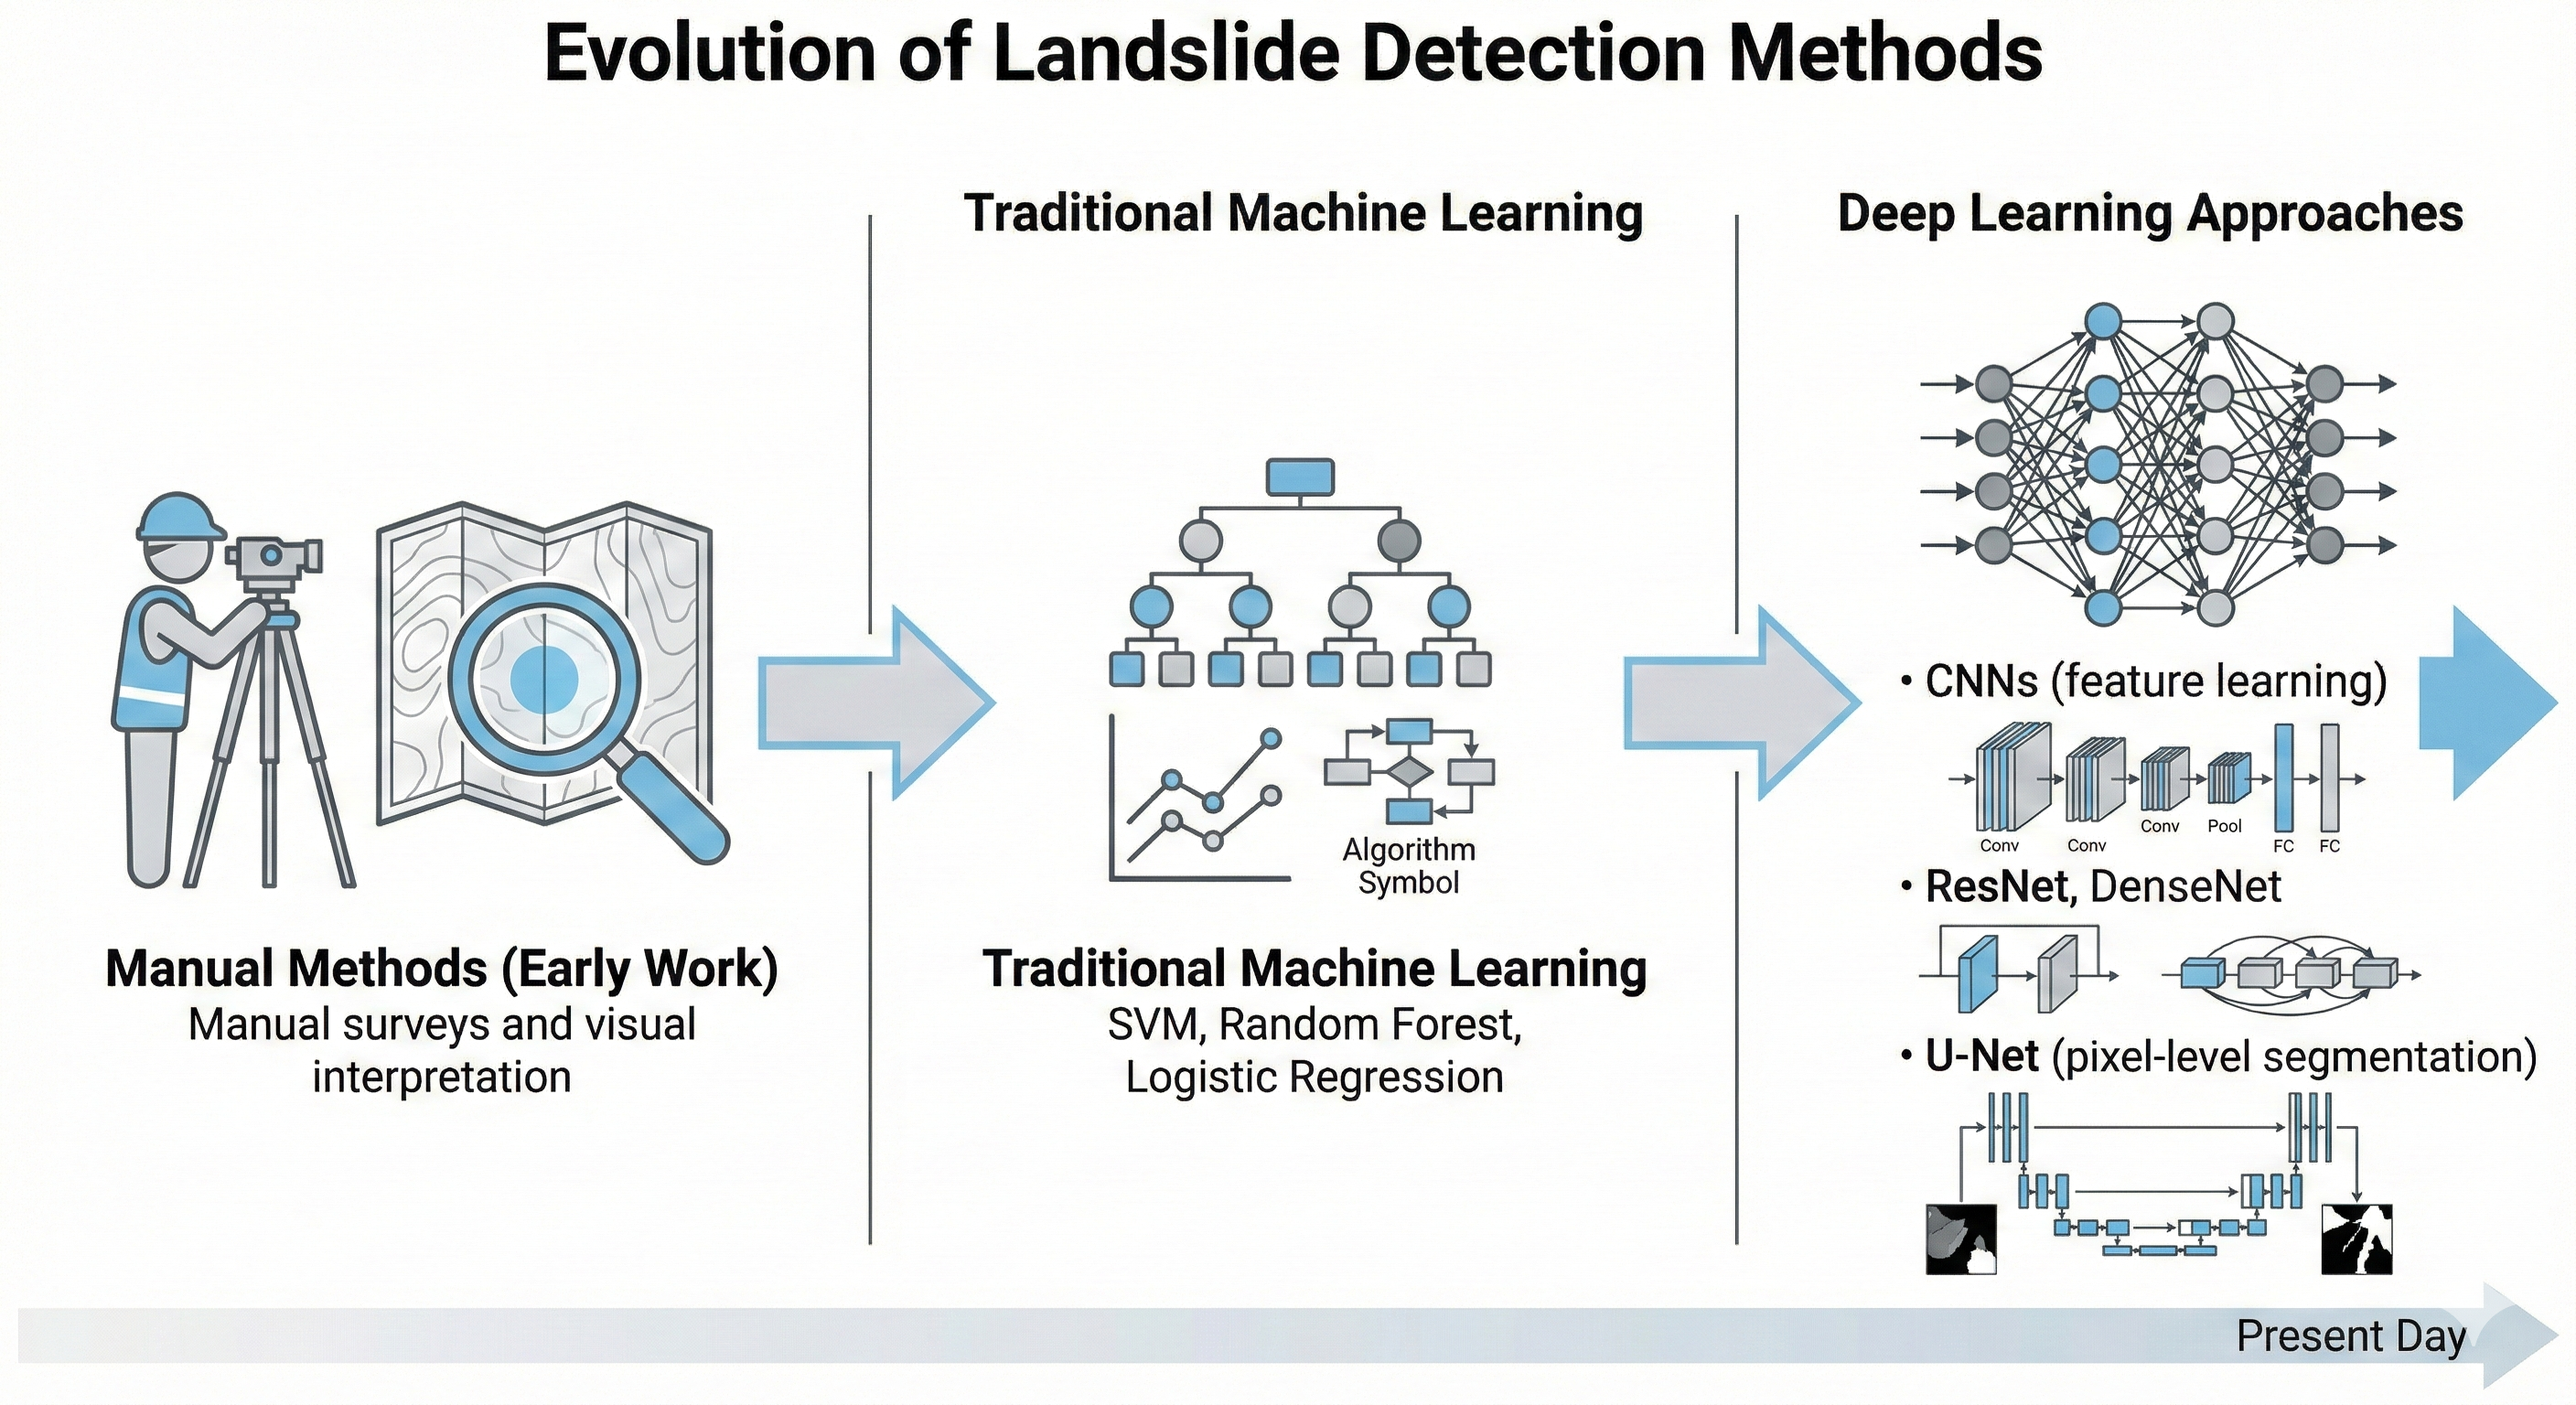
\includegraphics[width=0.9\linewidth]{Previous_work.png}
		\end{center}
		
		\vspace{0.3cm}
		
		% -------- SHORT TEXT (BOTTOM) --------
		\begin{itemize}
			\item Landslide detection methods evolved from manual surveys to machine learning and deep learning approaches.
			\item Deep learning models enable automatic and robust feature learning compared to traditional methods.
		\end{itemize}
		
	\end{frame}
	
	
	\begin{frame}{Limitations of Previous Work}
		\begin{itemize}
			\item Severe class imbalance in landslide datasets.
			\item Deep models overfit due to limited landslide samples.
			\item Underutilization of multispectral satellite data.
			\item Bias in fully connected classifiers.
		\end{itemize}
	\end{frame}
	% ---------- NEED FOR IMPROVEMENT ----------
	\begin{frame}{Need for Improvement}
		
		% -------- IMAGE (TOP) --------
		\begin{center}
			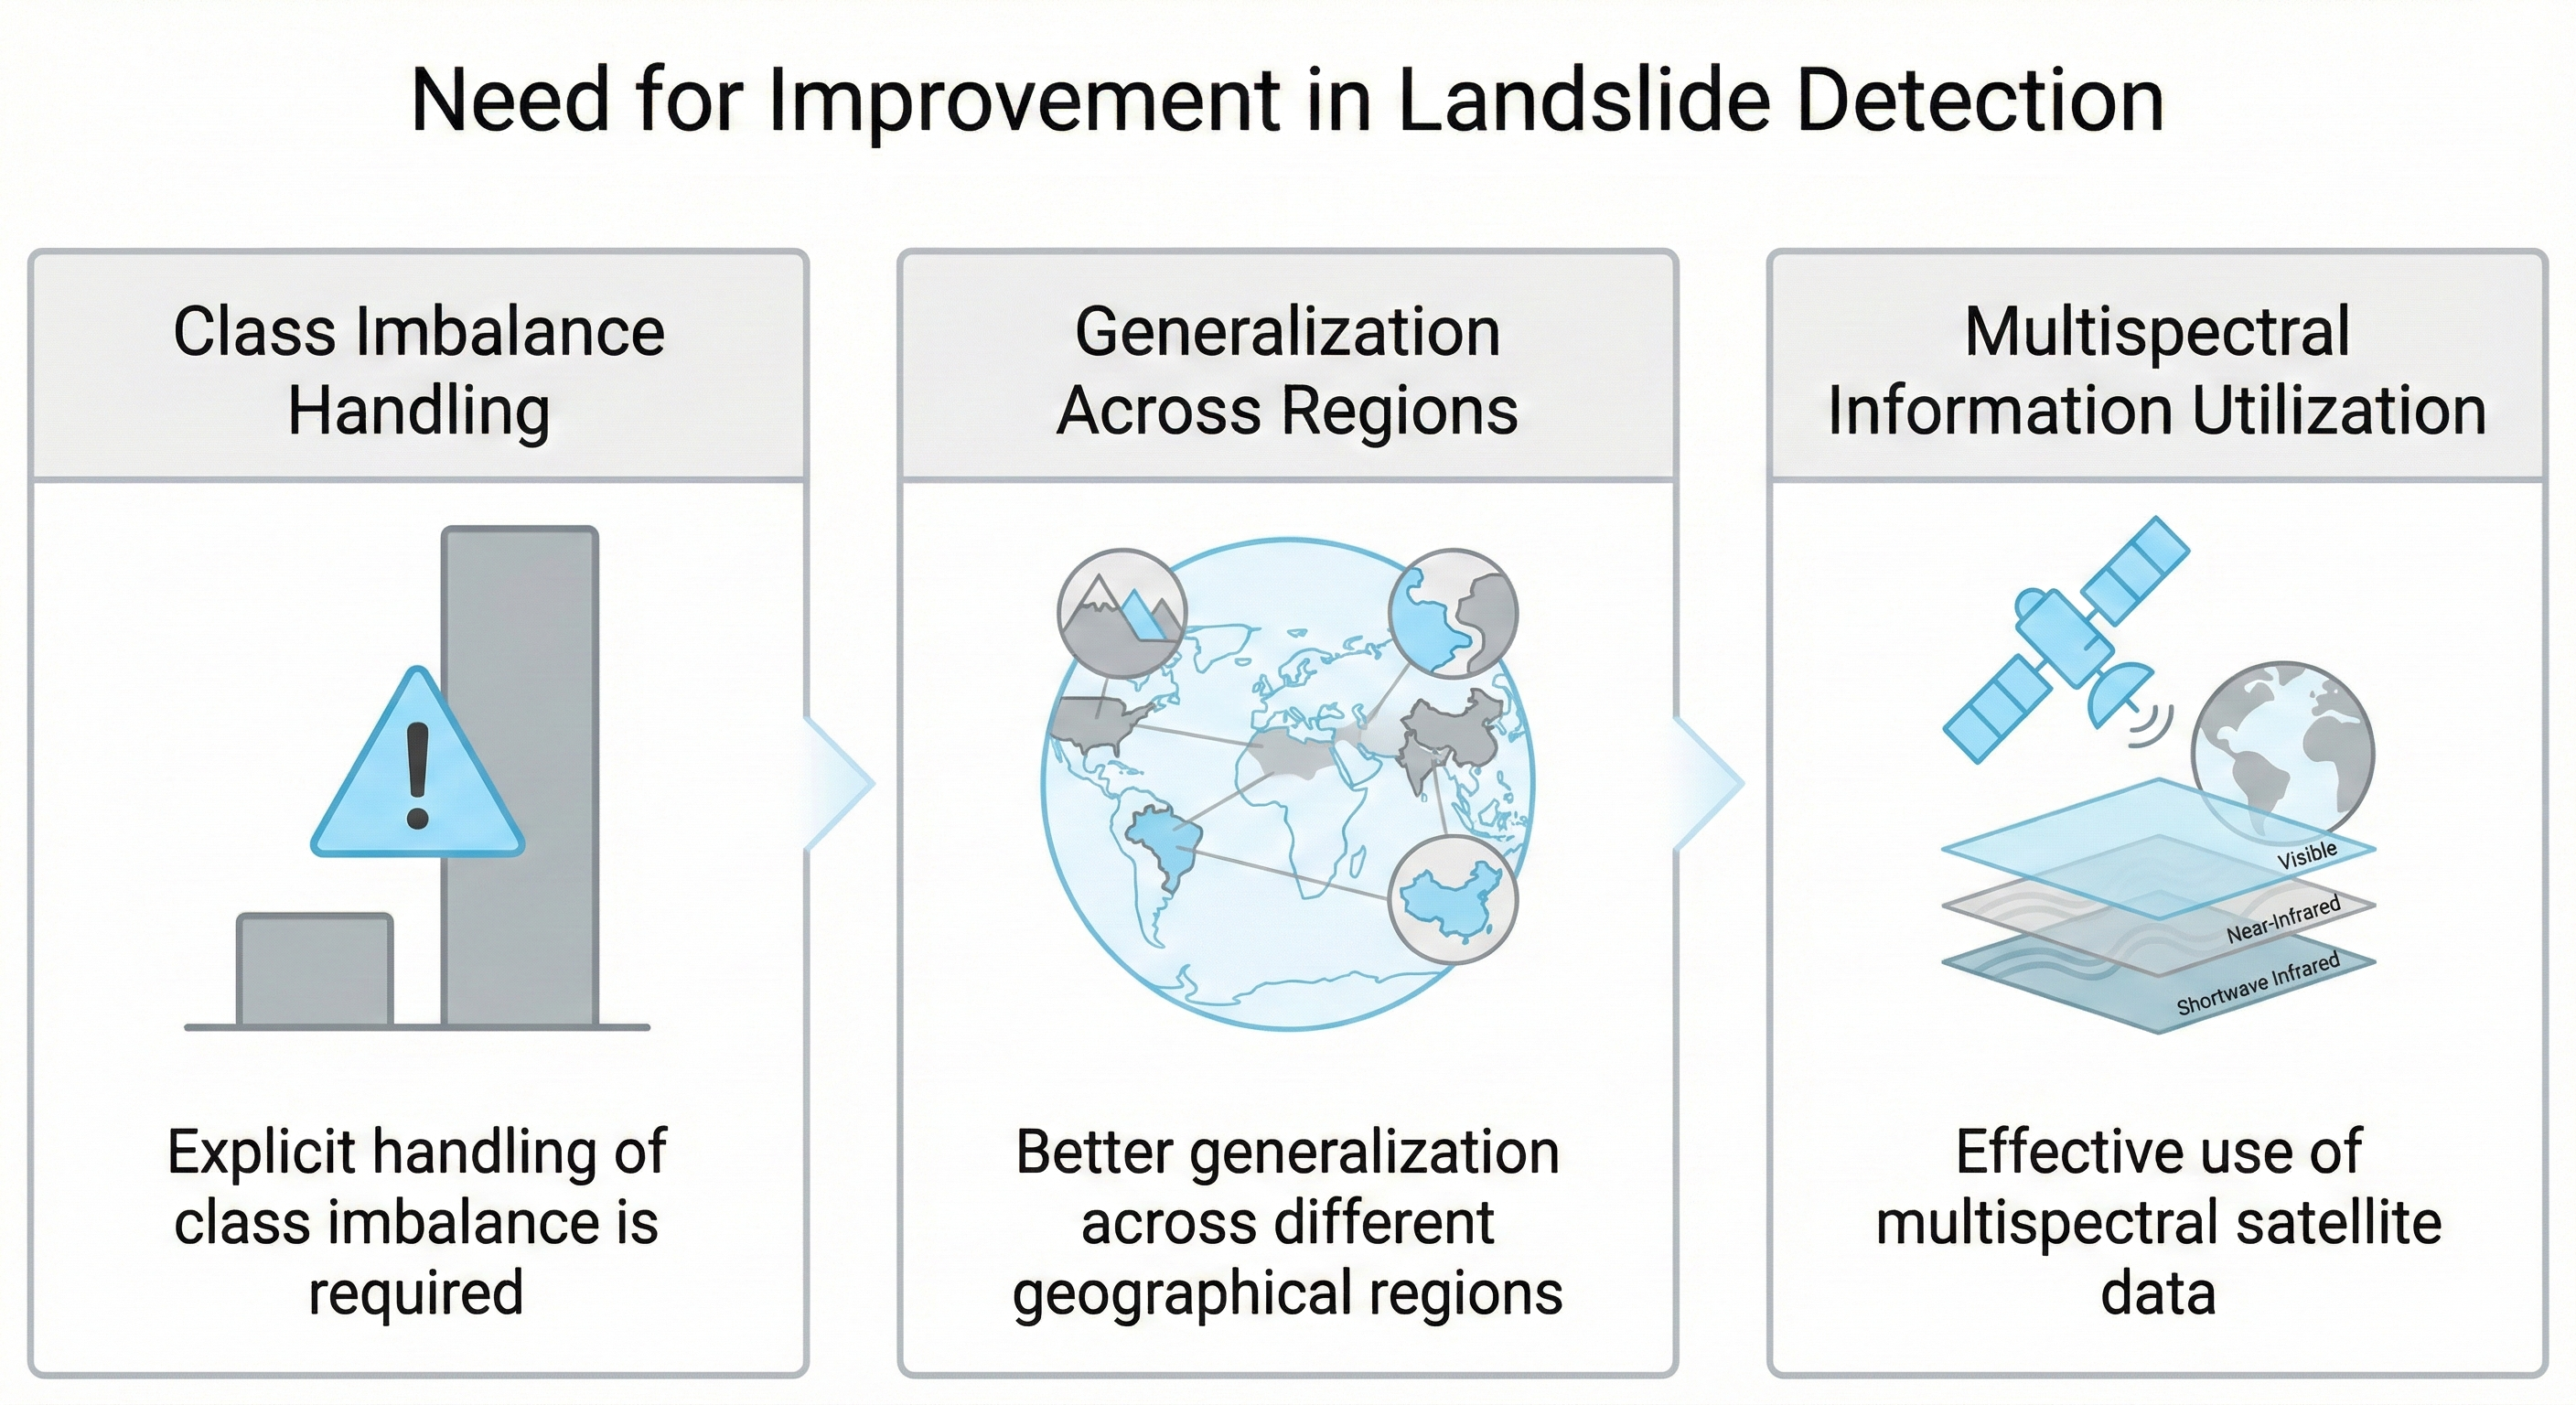
\includegraphics[width=0.9\linewidth]{Need_for_improvement.png}
		\end{center}
		
		\vspace{0.3cm}
		
		% -------- SHORT CAPTION (BOTTOM) --------
		\begin{itemize}
			\item Existing methods lack effective class imbalance handling and generalization.
			\item Improved utilization of multispectral data is essential for robust landslide detection.
		\end{itemize}
		
	\end{frame}
	
	
	% =================================================
	% DATASET
	% =================================================
	\section{Dataset Preparation}
	
	\begin{frame}{Dataset Description}
		\begin{itemize}
			\item Multispectral satellite dataset from \textbf{Zindi Africa}.
			\item Acquired via Landslide Detection competition.
			\item Each sample:
			\begin{itemize}
				\item $64 \times 64$ pixels
				\item 12 spectral bands
				\item Stored in \texttt{.npy} format
			\end{itemize}
			\item Two classes: Landslide and Non-landslide.
		\end{itemize}
	\end{frame}
	
% ---------- CHALLENGES IN THE DATASET ----------
\begin{frame}{Challenges in the Dataset}
	
	% -------- IMAGE (TOP) --------
	\begin{center}
		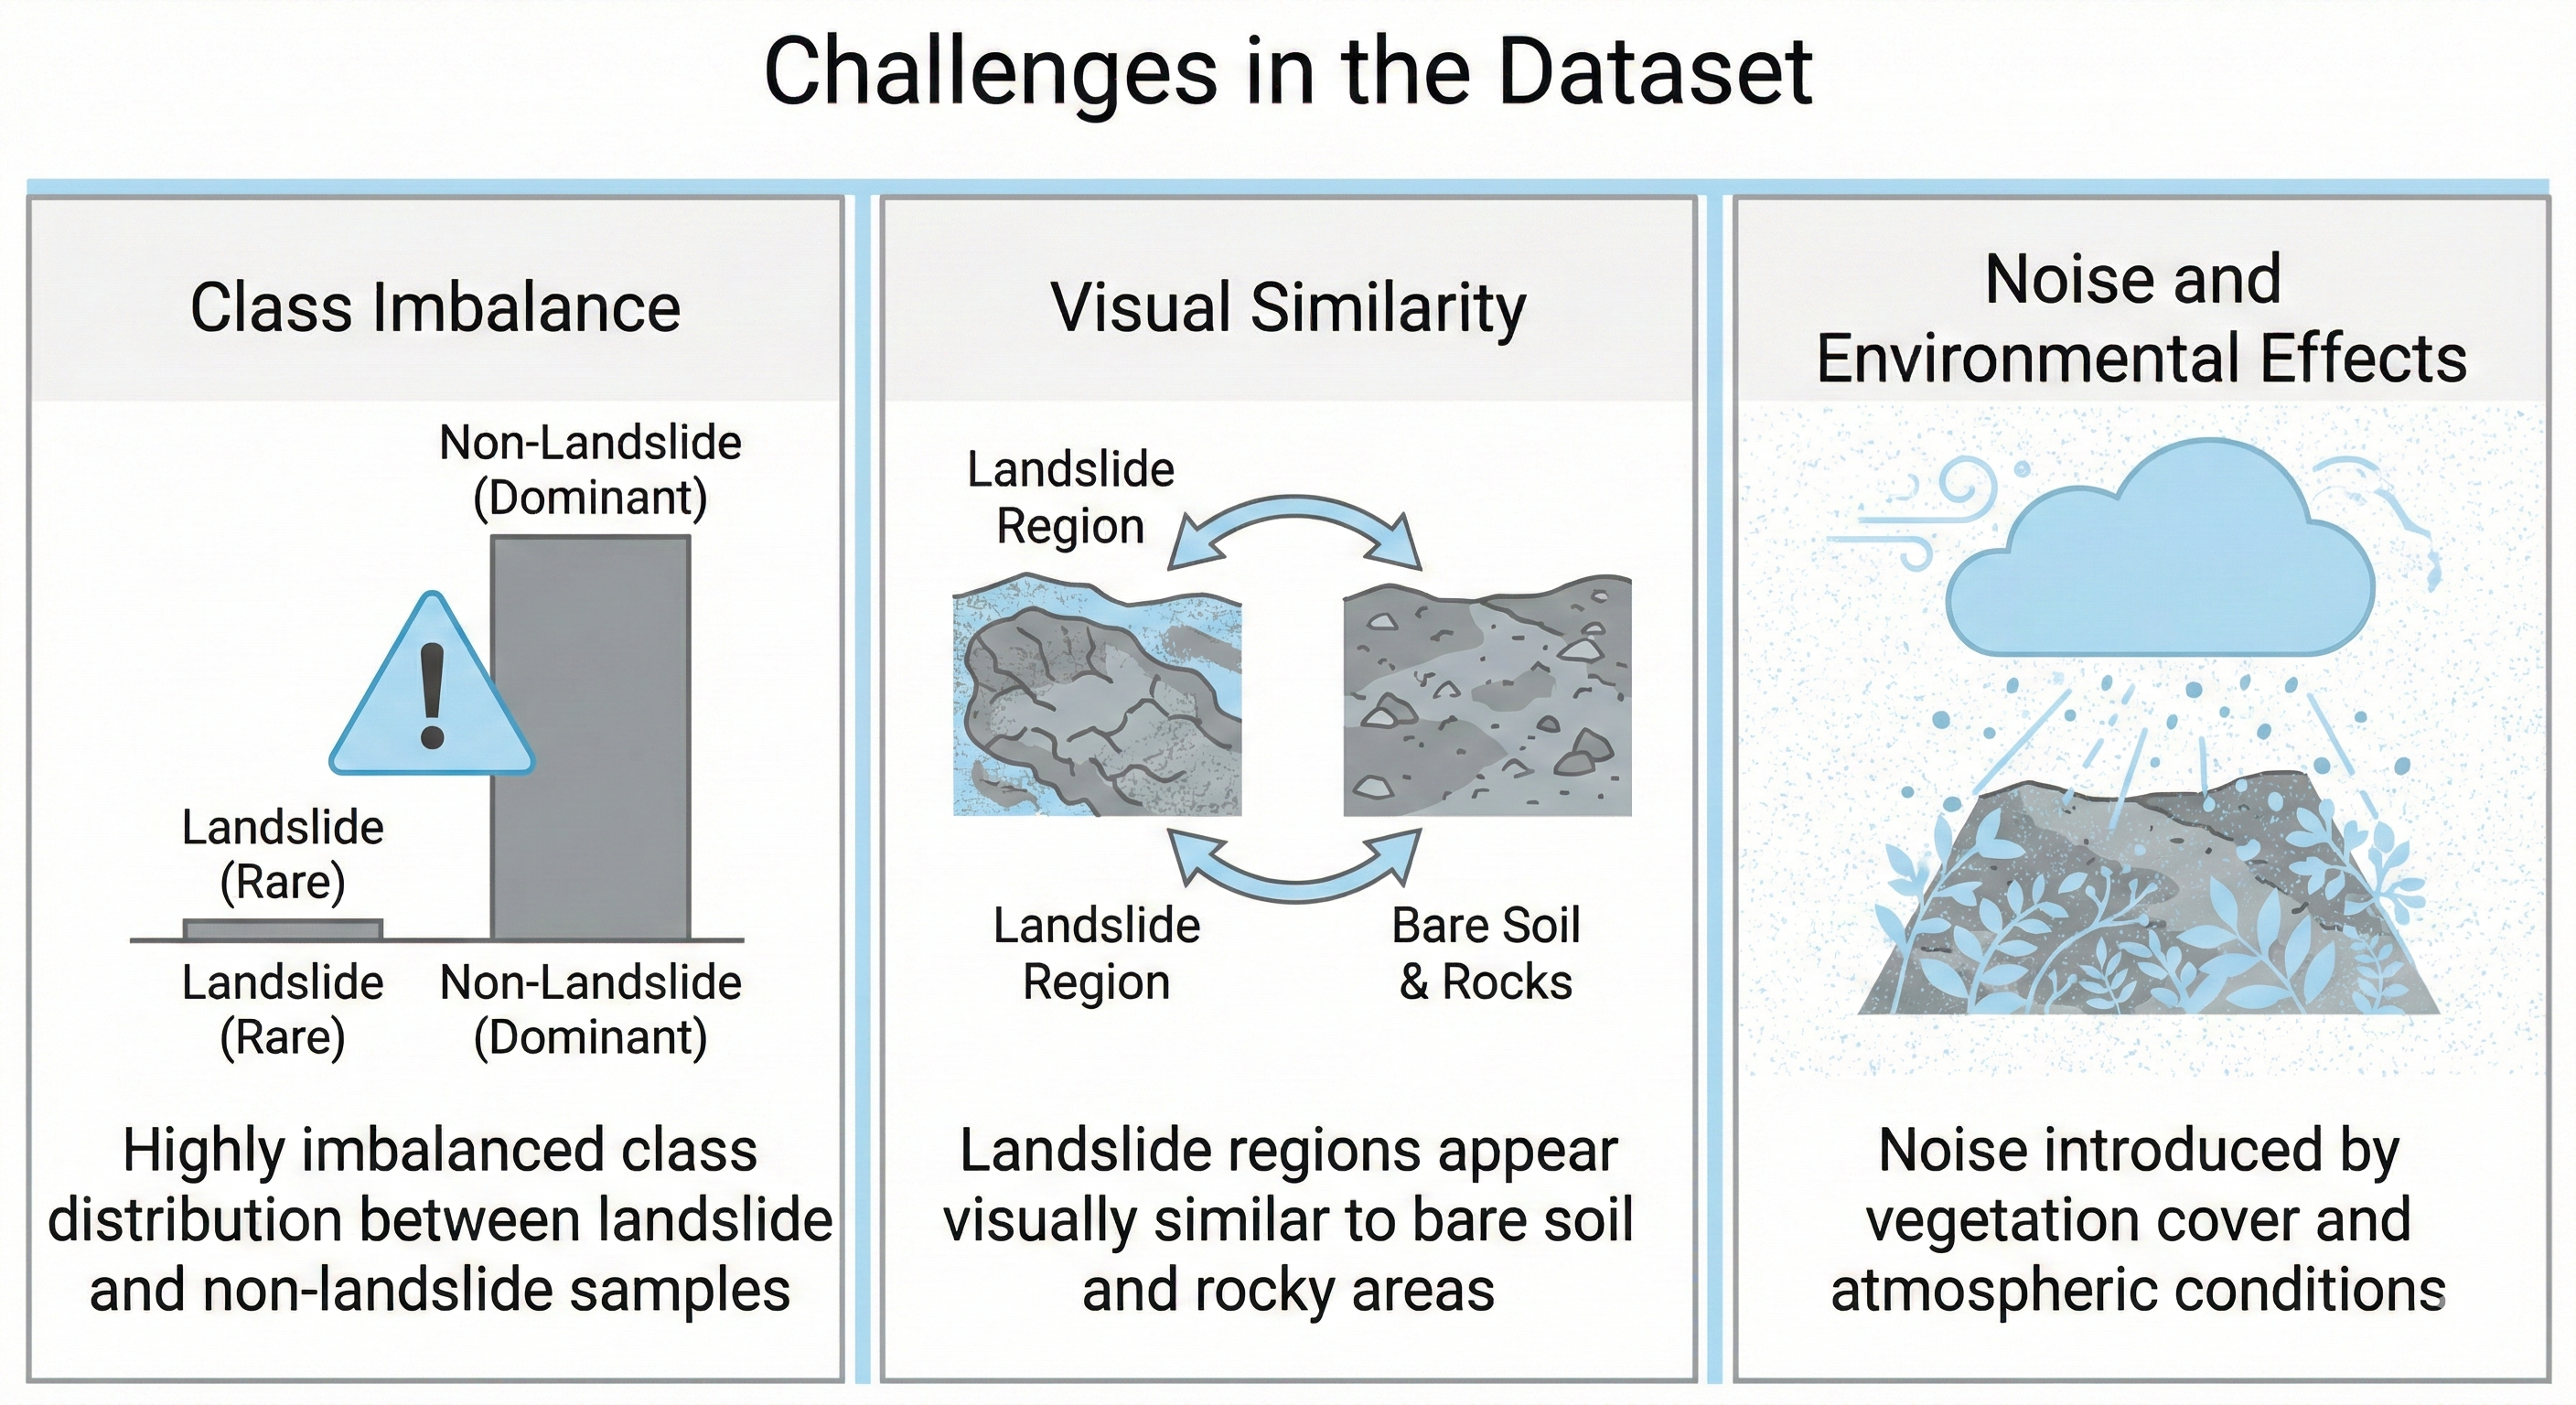
\includegraphics[width=0.9\linewidth]{Challenges.png}
	\end{center}
	
	\vspace{0.3cm}
	
	% -------- SHORT CAPTION (BOTTOM) --------
	\begin{itemize}
		\item The dataset suffers from class imbalance, visual ambiguity, and environmental noise.
		\item These challenges motivate robust data balancing and deep feature learning approaches.
	\end{itemize}
	
\end{frame}

	% =================================================
	% METHODOLOGY (UP TO FEATURE EXTRACTION)
	% =================================================
% =================================================
% METHODOLOGY
% =================================================
\section{Methodology}

% ---------- METHODOLOGY OVERVIEW ----------
\begin{frame}{Methodology Overview}
	\begin{itemize}
		\item Input multispectral satellite images.
		\item Preprocessing and normalization of raw data.
		\item Handling class imbalance using offline SMOTE.
		\item Creation of a balanced training dataset.
		\item Deep feature extraction using EfficientNetV2-Large.
	\end{itemize}
\end{frame}

	% =================================================
	% CLASS IMBALANCE HANDLING
	% =================================================
% =================================================
% CLASS IMBALANCE HANDLING
% =================================================
\section{Class Imbalance Handling}

% ---------- CLASS IMBALANCE PROBLEM ----------
\begin{frame}{Class Imbalance Problem}
	\begin{itemize}
		\item Landslide datasets are highly imbalanced in nature.
		\item Non-landslide samples significantly outnumber landslide samples.
		\item This imbalance leads to:
		\begin{itemize}
			\item Biased learning toward majority class
			\item Poor representation of landslide regions
		\end{itemize}
		\item Addressing class imbalance is essential before training deep models.
	\end{itemize}
\end{frame}



% ---------- OFFLINE SMOTE FOR DATASET BALANCING ----------
\begin{frame}{Offline SMOTE for Dataset Balancing}
	
	% -------- IMAGE (TOP) --------
	\begin{center}
		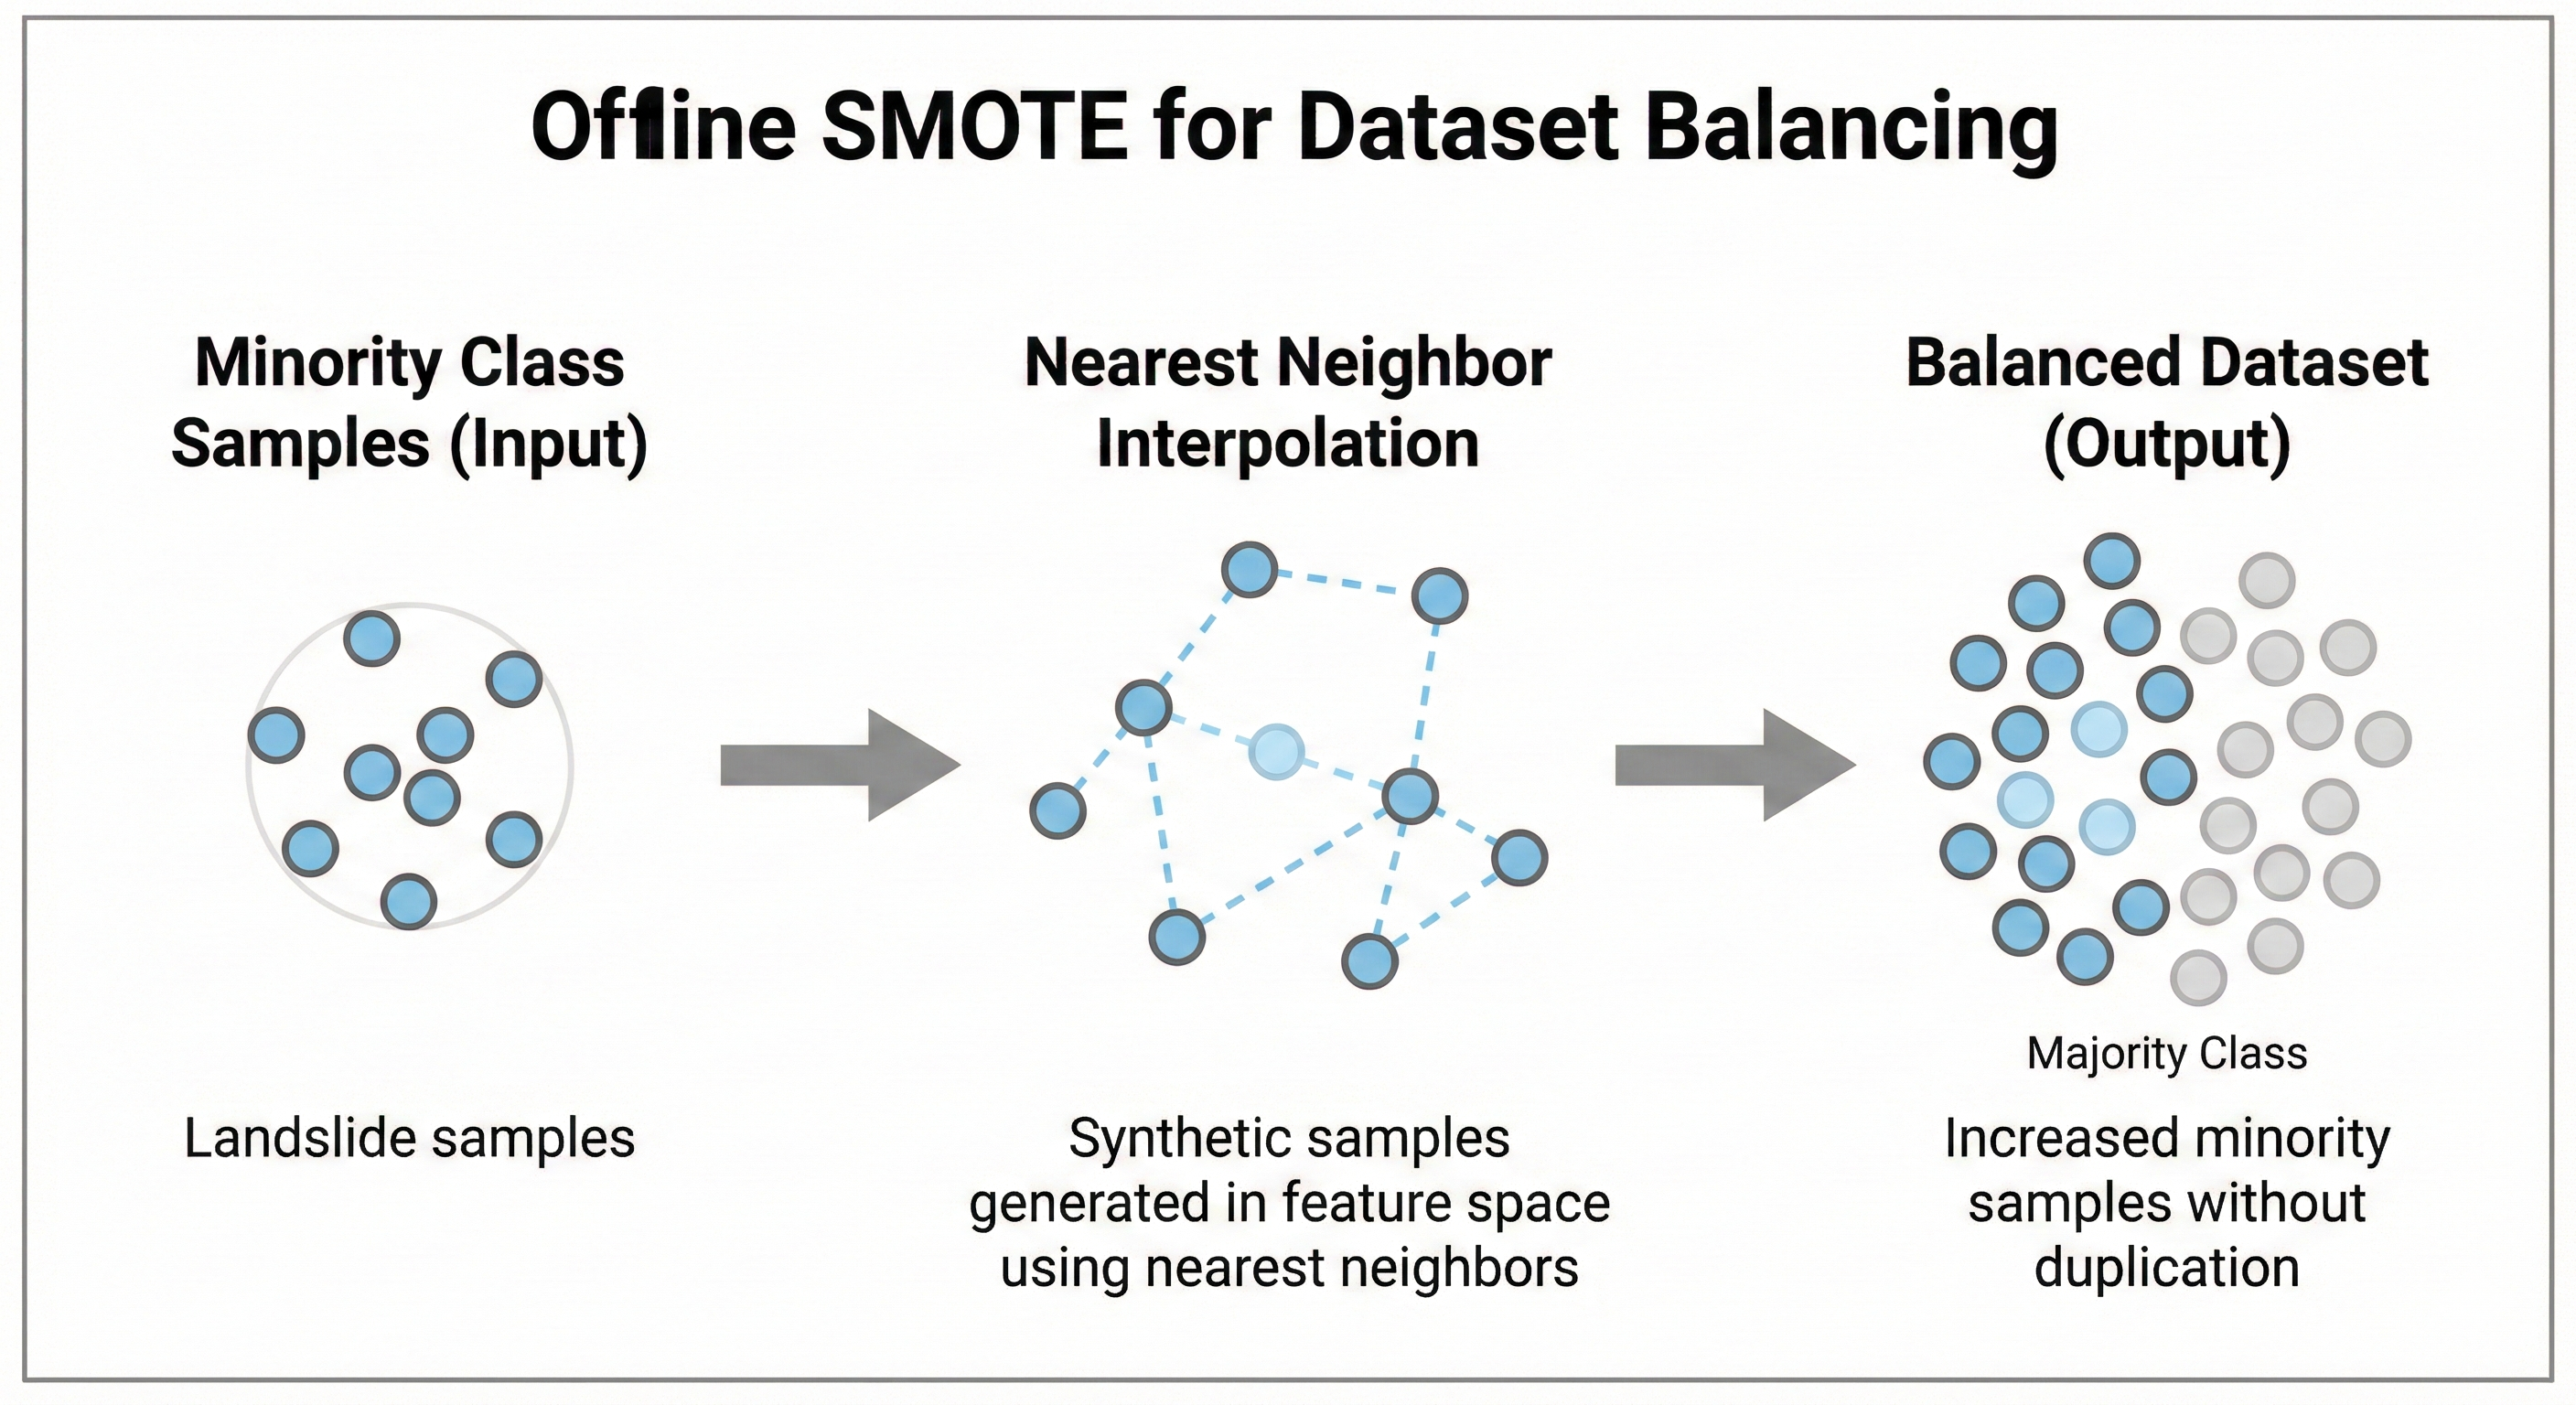
\includegraphics[width=1\linewidth]{Offline_smote_flow.png}
	\end{center}
	
	\vspace{0.3cm}
	
	% -------- SHORT DESCRIPTION (BOTTOM) --------
	\begin{itemize}
		\item SMOTE generates synthetic landslide samples by interpolating between nearest neighbors.
	\end{itemize}
	
\end{frame}

	% ---------- BALANCED DATASET FOR FEATURE LEARNING ----------
	\begin{frame}{Balanced Dataset for Feature Learning}
		
		% -------- IMAGE (TOP) --------
		\begin{center}
			\includegraphics[width=0.9\linewidth]{smote_generation_balanced.png}
		\end{center}
		
		\vspace{0.3cm}
		
		% -------- SHORT CAPTION (BOTTOM) --------
		\begin{itemize}
			\item After applying SMOTE, landslide and non-landslide classes are better balanced.
			
		\end{itemize}
		
	\end{frame}
	

	% =================================================
	% FEATURE EXTRACTION & EFFICIENTNETV2 ARCHITECTURE
	% =================================================
	
	% ---------- FEATURE EXTRACTION (CONCEPT) ----------
	\begin{frame}{Feature Extraction}
		\begin{itemize}
			\item Feature extraction transforms raw multispectral images into meaningful representations.
			\item Deep features are automatically learned from data without manual design.
			\item Extracted features capture:
			\begin{itemize}
				\item Spatial information such as texture and shape
				\item Spectral information from multiple satellite bands
			\end{itemize}
			\item These features are more robust than traditional handcrafted features.
		\end{itemize}
	\end{frame}

	
	% ---------- WHY CNNs FOR FEATURE EXTRACTION ----------
	\begin{frame}{Why CNNs for Feature Extraction}
		\begin{itemize}
			\item Convolutional Neural Networks (CNNs) are well-suited for image-based tasks.
			\item CNNs learn hierarchical features:
			\begin{itemize}
				\item Low-level features: edges and textures
				\item Mid-level features: regions and patterns
				\item High-level features: semantic representations
			\end{itemize}
			\item Local connectivity and weight sharing improve generalization.
		\end{itemize}
	\end{frame}
	% ---------- CNN FEATURE HIERARCHY ----------
	\begin{frame}{CNN Feature Hierarchy}
		\begin{center}
			% Conceptual illustration of CNN feature hierarchy
			\includegraphics[width=0.85\linewidth]{cnn_architecture.png}
		\end{center}
		
	\end{frame}
	
	
	% ---------- EFFICIENTNETV2 ARCHITECTURE OVERVIEW ----------
	\begin{frame}{EfficientNetV2 Architecture Overview}
		\begin{itemize}
			\item EfficientNetV2 is a modern and efficient deep convolutional architecture.
			\item It follows a compound scaling strategy to balance:
			\begin{itemize}
				\item Network depth
				\item Network width
				\item Input resolution
			\end{itemize}
			\item Designed for faster training and improved accuracy.
			\item Uses Fused-MBConv and MBConv blocks for efficient feature learning.
		\end{itemize}
	\end{frame}
	% ---------- EFFICIENTNETV2 ARCHITECTURE (REFERENCE IMAGE) ----------
	\begin{frame}{EfficientNetV2 Architecture}
		\begin{center}
			% Architecture image sourced from ResearchGate
			\includegraphics[width=0.30\linewidth]{Architecture-of-efficientNetv2_researchgate.png}
		\end{center}
	\end{frame}
	
	% ---------- EFFICIENTNETV2 FOR MULTISPECTRAL DATA ----------
	\begin{frame}{EfficientNetV2 for Multispectral Feature Extraction}
		\begin{itemize}
			\item Original EfficientNetV2 is designed for 3-channel RGB images.
			\item In this work, the input layer is modified to support:
			\begin{itemize}
				\item 12-channel multispectral satellite images
			\end{itemize}
			\item Enables effective utilization of terrain, vegetation, and soil information.
			\item EfficientNetV2 acts as a robust deep feature extractor for landslide detection.
		\end{itemize}
	\end{frame}
	
	% ---------- EFFICIENTNETV2 ARCHITECTURE IMAGE ----------
	\begin{frame}{EfficientNetV2-Large Architecture}
		\begin{center}
			\includegraphics[width=0.95\linewidth]{efficientnetv2_architecture.png}
		\end{center}
	\end{frame}
		% ---------- FEATURE EXTRACTION VISUALIZATION ----------
	\begin{frame}{Feature Extraction Process Visualization}
		
		\begin{center}
			\includegraphics[width=0.95\linewidth]{feature_extraction_4panel.png}
		\end{center}
		
		\vspace{0.2cm}
		
		\begin{center}
			\small
			\textit{Step-wise visualization of feature extraction in EfficientNetV2:
				Input multispectral image $\rightarrow$ Early convolutional features $\rightarrow$
				Intermediate abstract features $\rightarrow$ High-level feature embedding}
		\end{center}
		
	\end{frame}
	% ---------- FEATURE EXTRACTION EXPLANATION ----------
	\begin{frame}{Explanation of Feature Extraction Stages}
		
		\begin{itemize}
			\item \textbf{Input Image:}
			\begin{itemize}
				\item Represents a multispectral satellite patch used for landslide detection.
				\item Contains terrain and surface information across multiple spectral bands.
			\end{itemize}
			
			\item \textbf{Early Feature Maps:}
			\begin{itemize}
				\item Capture low-level patterns such as edges, textures, and local intensity variations.
				\item Useful for identifying abrupt terrain changes.
			\end{itemize}
			
			\item \textbf{Mid-Level Feature Maps:}
			\begin{itemize}
				\item Learn higher-order spatial structures and region-level patterns.
				\item Encode combinations of textures and terrain characteristics.
			\end{itemize}
			
			\item \textbf{High-Level Feature Embedding:}
			\begin{itemize}
				\item Obtained after global pooling in EfficientNetV2.
				\item Produces a compact feature vector used for final classification.
			\end{itemize}
		\end{itemize}
		
	\end{frame}
	
	% ---------- FEATURE EXTRACTION SUMMARY ----------
	\begin{frame}{Feature Extraction Summary}
		\begin{itemize}
			\item Multispectral images are processed using EfficientNetV2-Large.
			\item The network learns discriminative spatial and spectral features.
			\item Extracted deep features form the foundation for subsequent classification.
			\item This stage completes the core representation learning of the framework.
		\end{itemize}
	\end{frame}
	
	
	\begin{frame}{High-Level Framework}
		\begin{center}
			\includegraphics[width=0.95\linewidth]{model_architecture.png}
		\end{center}
		
	\end{frame}
	% =================================================
	% WORK COMPLETED SO FAR
	% =================================================
	\begin{frame}{Work Completed So Far}
		\begin{itemize}
			\item Studied the problem of landslide detection using satellite imagery.
			\item Reviewed existing literature and identified limitations of prior methods.
			\item Collected and analyzed multispectral satellite dataset from Zindi Africa.
			\item Performed dataset understanding and identified class imbalance issues.
			\item Designed the overall deep learning framework.
			\item Implemented feature extraction using EfficientNetV2-Large:
			\begin{itemize}
				\item Adapted the network for 12-channel multispectral input
				\item Extracted high-level spatial and spectral features
			\end{itemize}
			\item Completed the core representation learning stage of the project.
		\end{itemize}
	\end{frame}
	
	% =================================================
	% FUTURE WORK / REMAINING WORK
	% =================================================
	\begin{frame}{Future Work}
		\begin{itemize}
			\item Train the deep learning model with optimized hyperparameters.
			\item Integrate Support Vector Machine (SVM) for final classification.
			\item Perform extensive performance evaluation using:
			\begin{itemize}
				\item Accuracy, Precision, Recall, F1-score
			\end{itemize}
			\item Analyze results and compare with existing approaches.
			\item Prepare final documentation and presentation.
		\end{itemize}
	\end{frame}
	
\end{document}
